\section{Chapter 2}
\subsection{2.1}
\begin{itemize}
   \item[10.] Determine whether these statements are true or false.
         \begin{enumerate}[a.]
            \item $\emptyset \in \{\emptyset\} $
            \item $\emptyset \in \{\emptyset, \{\emptyset \}\}$
            \item $\{\emptyset\} \in \{\emptyset \}$
            \item $\{\emptyset\} \in \{\{\emptyset\}\}$
            \item $\{\emptyset\} \subset \{\emptyset, \{\emptyset\}\}$
            \item $\{\{\emptyset\}\} \subset \{\emptyset, \{\emptyset\}\}$
            \item $\{\{\emptyset\}\} \subset \{\{\emptyset\}, \{\emptyset\}\}$
         \end{enumerate}
         \answer
         \begin{enumerate}[a.]
            \item True
            \item True
            \item False
            \item True
            \item True
            \item True
            \item False
         \end{enumerate}
   \item[16.] Use a Venn diagram to illustrate the relationship $A \subset B$ and $A \subset C$\\
         \answer \\
         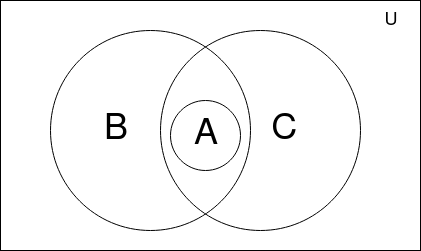
\includegraphics[scale=.7]{2_1_16_VennDiagram}
   \item[24.] Determine whether each of these sets is the power set of a set, where a and b are distinct elements.
         \begin{enumerate}[a.]
            \item $\emptyset$
            \item $\{\emptyset, \{a\}\}$
            \item $\{\emptyset, \{a\}, \{\emptyset, a\}\}$
            \item $\{\emptyset, \{a\}, \{b\}, \{a, b\}\}$
         \end{enumerate}
         \answer
         \begin{enumerate}
            \item No
            \item Yes, $P(\{a\})$
            \item No
            \item Yes, $P(\{a, b\})$
         \end{enumerate}
   \item [32.] Let $A = \{a, b, c\}, B = \{x, y\}, \text{and} C = \{0, 1\}$. Find
         \begin{enumerate}[a.]
            \item $A \times B \times C$.
            \item $C \times B \times A$.
            \item $C \times A \times B$.
            \item $B \times B \times B$.
         \end{enumerate}
         \answer
         \begin{enumerate}[a.]
            \item $A \times B \times C = \{(a, x, 0), (a, x, 1), (a, y, 0), (a, y, 1), (b, x, 0), (b, x, 1), (b, y, 0), (b, y, 1), (c, x, 0), (c, x, 1), (c, y, 0), (c, y, 1)\}$
            \item $C \times B \times A = \{(0, x, a), (0, x, b), (0, x, c), (0, y, a), (0, y, b), (0, y, c), (1, x, a), (1, x, b), (1, x, c), (1, y, a), (1, y, b), (1, y, c)\}$
            \item $C \times A \times B = \{(0, a, x), (0, a, y), (0, b, x), (0, b, y), (0, c, x), (0, c, y), (1, a, x), (1, a, y), (1, b, x), (1, b, y), (1, c, x), (1, c, y)\}$
            \item $B \times B \times B = \{(x, x, x), (x, x, y), (x, y, x), (x, y, y), (y, x, x), (y, x, y), (y, y, x), (y, y, y)\}$
         \end{enumerate}
\end{itemize}

\subsection{2.2}
\begin{itemize}
   \item[2.] Suppose that $A$ is the set of sophomores at your school and $B$ is the set of students in discrete mathematics at your school. Express each of these sets in terms of $A$ and $B$.
         \begin{enumerate}[a.]
            \item The set of sophomores taking discrete mathematics in your school
            \item The set of sophomores at your school who are not taking discrete mathematics
            \item The set of students at your school who either are sophomores or are taking discrete mathematics
            \item The set of students at your school who either are not sophomores or are not taking discrete mathematics
         \end{enumerate}
         \begin{enumerate}[a.]
            \item $A \cap B$
            \item $A - B$
            \item $A \cup B$
            \item $\overline{A} \cup \overline{B}$
         \end{enumerate}
   \item[4.] Let $A = \{a, b, c, d, e\} \text{and} B = \{a, b, c, d, e, f, g, h\}.$ \\
         Find.
         \begin{enumerate}[a.]
            \item $A \cup B$
            \item $A \cap B$
            \item $A - B$
            \item $B - A$
         \end{enumerate}
         \answer
         \begin{enumerate}[a.]
            \item $\{a, b, c, d, e, f, g, h\}$
            \item $\{a, b, c, d, e\}$
            \item $\emptyset$
            \item $\{f, g, h\}$
         \end{enumerate}
   \item[26.] Draw the Venn diagrams for each of these combinations of the sets A, B, and C.
         \begin{enumerate}[a.]
            \item $A \cap (B \cup C)$
            \item $\overline{A} \cap \overline{B} \cap \overline{C}$
            \item $(A - B) \cup (A - C) \cup (B - C)$
         \end{enumerate}
         \begin{enumerate}[a.]
            \item \vspace{3mm} 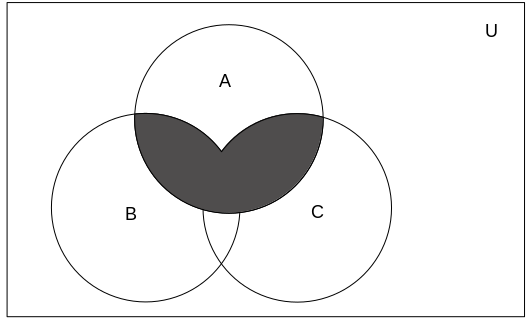
\includegraphics[scale=0.8]{2_2_26_a_VennDiagram}
            \item \vspace{3mm} 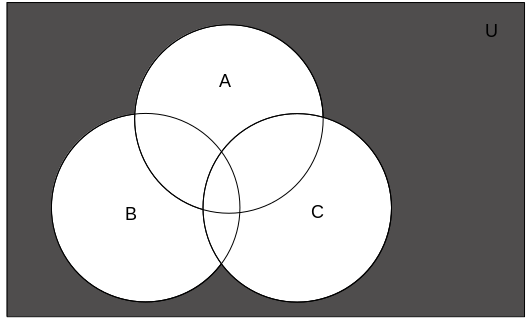
\includegraphics[scale=0.8]{2_2_26_b_VennDiagram}
            \item \vspace{3mm} 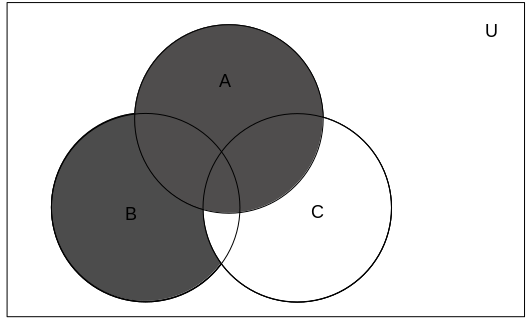
\includegraphics[scale=0.8]{2_2_26_c_VennDiagram}
         \end{enumerate}
\end{itemize}

\subsection{2.3}
\begin{itemize}
   \item[8.]Find these values.
         \begin{enumerate}[a.]
            \item $\lfloor 1.1 \rfloor$
            \item $\lceil 1.1 \rceil$
            \item $\lfloor -0.1 \rfloor$
            \item $\lceil -0.1 \rceil$
            \item $\lceil 2.99 \rceil$
            \item $\lfloor -2.99 \rfloor$
            \item $\lfloor \frac{1}{2} + \lceil \frac{1}{2} \rceil \rfloor$
            \item $\lceil \lfloor \frac{1}{2} \rfloor + \lceil \frac{1}{2} \rceil + \frac{1}{2} \rceil $
         \end{enumerate}
         \answer
         \begin{enumerate}[a.]
            \item 1
            \item 2
            \item -1
            \item 0
            \item 3
            \item -2
            \item 1
            \item 2
         \end{enumerate}
   \item[10.] Determine whether each of these functions from $\{a, b, c, d\}$ to itself is one-to-one.
         \begin{enumerate}[a.]
            \item $f (a) = b, f (b) = a, f (c) = c, f (d) = d$
            \item $f (a) = b, f (b) = b, f (c) = d, f (d) = c$
            \item $f (a) = d, f (b) = b, f (c) = c, f (d) = d$
         \end{enumerate}
         \answer
         \begin{enumerate}[a.]
            \item Yes
            \item No
            \item No
         \end{enumerate}

   \item[12.]Determine whether $f : \mathbb{Z} \times \mathbb{Z} \to \mathbb{Z}$ is onto if
         \begin{enumerate}[a.]
            \item $f(m,n) = 2m - n$
            \item $f(m,n) = m^2 - n^2$
            \item $f(m,n) = m + n + 1$
            \item $f(m,n) = \lvert m \rvert - \lvert n \rvert$
            \item $f(m,n) = m^2 - 4$
         \end{enumerate}
         \answer
         \begin{enumerate}[a.]
            \item Yes, to get any $x \in \mathbb{Z}$ you can do $f(0, -x)$
            \item No, for example it cannot map to 1
            \item Yes, to get any $x \in \mathbb{Z}$ you can do $f(x, -1)$
            \item Yes, to get any $x \in \mathbb{Z}^+$ you can do $f(x, 0)$ and to get any $y \in \mathbb{Z}^-$ you can do $f(0, y)$ and to get $f(m,n) = 0$ you can do $f(0, 0)$.
            \item No, function cannot map to anything less than -4.
         \end{enumerate}

   \item[20] Give an example of a function from $\mathbb{N}$ to $\mathbb{N}$ that is
         \begin{enumerate}[a.]
            \item One-to-one, but not onto.
            \item Onto, but not one-to-one.
            \item Both onto and one-to-one.(Not the identity)
            \item Neither one-to-one or onto
         \end{enumerate}
         \answer
         \begin{enumerate}[a.]
            \item $f(x) = x+1$
            \item $f(x) = \begin{cases}
                        0     & x = 0    \\
                        x - 1 & x \geq 1
                     \end{cases}$
            \item $f(x) = \begin{cases}
                        1 & x = 0 \\
                        0 & x = 1 \\
                        x & x > 1 \\
                     \end{cases}$
            \item $f(x) = 1$
         \end{enumerate}
\end{itemize}

\subsection{2.4}
\begin{itemize}
   \item[2.] What is the term $a_8$ of the sequence $\{a_n\}$ if $a_n$ equals
         \begin{enumerate}[a.]
            \item $2^{n-1}$
            \item 7
            \item $1 + (-1)^n$
            \item $-(-2)^n$
         \end{enumerate}
         \answer
         \begin{enumerate}[a.]
            \item 128
            \item 7
            \item 2
            \item -256
         \end{enumerate}
   \item[4.] What are the terms $a_0$ , $a_1$ , $a_2$ , and $a_3$ of the sequence $\{a_n\}$, where $a_n$ equals
         \begin{enumerate}[a.]
            \item $(-2)^n$
            \item 3
            \item $7 + 4^n$
            \item $2^n + (-2)^n$
         \end{enumerate}
         \answer
         \begin{enumerate}[a.]
            \item 1, -2, 4, -8
            \item 3, 3, 3, 3
            \item 8, 11, 24, 71
            \item 2, 0, 8, 0
         \end{enumerate}
   \item[6.] List the first 10 terms of each of these sequences.
         \begin{enumerate}[a.]
            \item the sequence obtained by starting with 10 and obtaining each term by subtracting 3 from the previous term
            \item the sequence whose nth term is the sum of the first n positive integers
            \item the sequence whose nth term is $3^n - 2^n$
            \item the sequence whose nth term is  $\lfloor \sqrt{n} \rfloor$
            \item the sequence whose first two terms are 1 and 5 and each succeeding term is the sum of the two previous terms
            \item the sequence whose nth term is the largest integer whose binary expansion (defined in Section 4.2) has n bits (Write your answer in decimal notation.)
            \item the sequence whose terms are constructed sequentially as follows: start with 1, then add 1, then multiply by 1, then add 2, then multiply by 2, and so on
            \item the sequence whose nth term is the largest integer $k$ such that $k! \leq n$
         \end{enumerate}
         \answer
         \begin{enumerate}[a.]
            \item 10, 7, 4, 1, -2, -5, -8, -11, -14, -17
            \item 1, 3, 6, 10, 15, 21, 28, 36, 45, 55
            \item 1, 5, 19, 65, 211, 665, 2059, 6305, 19171, 58025
            \item 1, 1, 1, 2, 2, 2, 2, 2, 3, 3
            \item 1, 5, 6, 11, 17, 28, 45, 73, 118, 191
            \item 1, 3, 7, 15, 31, 63, 127, 255, 511, 1023
            \item 1, 2, 2, 4, 8, 11, 33, 37, 148, 153
            \item 1, 2, 2, 2, 2, 3, 3, 3, 3, 3
         \end{enumerate}
\end{itemize}

\subsection{2.6}
\begin{itemize}
   \item[2.] Find $A + B$
         \begin{enumerate}[a.]
            \item
                  $A = \begin{bmatrix}
                        1  & 0  & 4  \\
                        -1 & 2  & 2  \\
                        0  & -2 & -3
                     \end{bmatrix}$
                  $B = \begin{bmatrix}
                        -1 & 3  & 5 \\
                        2  & 2  & 3 \\
                        2  & -3 & 0
                     \end{bmatrix}$
            \item
                  $A = \begin{bmatrix}
                        -1 & 0  & 5 & 6  \\
                        -4 & -3 & 5 & -2
                     \end{bmatrix}$
                  $B = \begin{bmatrix}
                        -3 & 9  & -3 & 4 \\
                        0  & -2 & -1 & 2
                     \end{bmatrix}$
         \end{enumerate}
         \answer
         \begin{enumerate}[a.]
            \item
                  $A + B =  \begin{bmatrix}
                        0 & 3  & 9  \\
                        1 & 4  & 5  \\
                        2 & -5 & -3
                     \end{bmatrix}$
            \item
                  $A + B = \begin{bmatrix}
                        -4 & 9  & 2 & 10 \\
                        -4 & -5 & 4 & 0
                     \end{bmatrix}$
         \end{enumerate}
   \item[4.] Find the product AB, where
         \begin{enumerate}[a.]
            \item
                  $A = \begin{bmatrix}
                        1  & 0  & 1  \\
                        0  & -1 & -1 \\
                        -1 & 1  & 0
                     \end{bmatrix}$
                  $B = \begin{bmatrix}
                        0  & 1  & -1 \\
                        1  & -1 & 0  \\
                        -1 & 0  & 1
                     \end{bmatrix}$
            \item
                  $A = \begin{bmatrix}
                        1 & -3 & 0  \\
                        1 & 2  & 2  \\
                        2 & 1  & -1
                     \end{bmatrix}$
                  $B = \begin{bmatrix}
                        1  & -1 & 2 & 3  \\
                        -1 & 0  & 3 & -1 \\
                        -3 & -2 & 0 & 2
                     \end{bmatrix}$
            \item
                  $A = \begin{bmatrix}
                        0  & -1 \\
                        7  & 2  \\
                        -4 & -3
                     \end{bmatrix}$
                  $B = \begin{bmatrix}
                        4  & -1 & 2 & 3 & 0 \\
                        -2 & 0  & 3 & 4 & 1
                     \end{bmatrix}$
         \end{enumerate}
         \answer
         \begin{enumerate}[a.]
            \item
                  $AB = \begin{bmatrix}
                        -1 & 1  & 0  \\
                        0  & 1  & -1 \\
                        1  & -2 & 1
                     \end{bmatrix}$
            \item
                  $AB = \begin{bmatrix}
                        4  & -1 & -7 & 6 \\
                        -7 & -5 & 6  & 5 \\
                        -5 & 0  & 7  & 3
                     \end{bmatrix}$
            \item
                  $AB = \begin{bmatrix}
                        2   & 0  & -3  & -4  & -1 \\
                        24  & -7 & 20  & 29  & 2  \\
                        -10 & 4  & -17 & -24 & -3
                     \end{bmatrix}$ \vspace{3mm}
         \end{enumerate}
   \item[26.] Let $A = \begin{bmatrix} 1 & 1 \\ 0 & 1 \end{bmatrix} B = \begin{bmatrix} 0 & 1 \\ 1 & 0 \end{bmatrix}$

         Find
         \begin{enumerate}[a.]
            \item $A \lor B$.
            \item $A \land B$
            \item $A \odot B$.
         \end{enumerate}
         \answer
         \begin{enumerate}[a.]
            \item $A \lor B = \begin{bmatrix} 1 & 1 \\ 1 & 1 \end{bmatrix}$
            \item $A \land B = \begin{bmatrix} 0 & 1 \\ 0 & 0 \end{bmatrix}$
            \item $A \odot B = \begin{bmatrix} 1 & 1 \\ 1 & 0 \end{bmatrix}$
         \end{enumerate}
\end{itemize}
